\documentclass[a4paper,12pt]{report}
\usepackage[catalan]{varioref}
\usepackage{setspace}
\usepackage[margin=2.54cm]{geometry}
\usepackage{pdfpages}
\usepackage[utf8]{inputenc}
\usepackage[catalan]{babel}
\usepackage{graphicx,subcaption}
\usepackage{graphics}
\usepackage{lscape}
\usepackage{pdflscape}
\usepackage{float}
\usepackage{textcomp}
\usepackage{amsmath}
\usepackage{hyperref}
\usepackage{subcaption}
\usepackage{pgfplots}
\usepackage{tikz}
\usepackage{fancyvrb}
\usepackage{parskip}
\usepackage{changepage}
\usepackage{enumitem}
\usepackage{tcolorbox}
\usepackage[all]{hypcap}
\usepackage{xcolor}
\usepackage{listings}
\definecolor{green}{HTML}{228B22}
\definecolor{orange}{HTML}{FFC107}
\usepackage{color}
\definecolor{dkgreen}{rgb}{0,0.6,0}
\definecolor{gray}{rgb}{0.5,0.5,0.5}
\definecolor{mauve}{rgb}{0.58,0,0.82}
\lstset{escapeinside={<@}{@>}}

\hypersetup{
    colorlinks,
    citecolor=black,
    filecolor=black,
    linkcolor=black,
    urlcolor=blue
}


\lstset{frame=tb,
    language=python,
    aboveskip=3mm,
    belowskip=3mm,
    showstringspaces=false,
    columns=flexible,
    basicstyle={\small\ttfamily},
    numbers=none,
    numberstyle=\tiny\color{gray},
    keywordstyle=\color{blue},
    commentstyle=\color{dkgreen},
    stringstyle=\color{mauve},
    breaklines=true,
    breakatwhitespace=true, tabsize=3
}
\title{
	\begin{center}
	\vspace{3cm}
	
\includegraphics[width=11cm, height=3cm]{images/Logo-uoc.png}
	\end{center}
	\begin{center}
	\line(1,0){400}
	\end{center}		
	TIPOLOGIA I CICLE DE VIDA DE LES DADES\\
	\vspace{2mm}
	\Large PAC2: Introducció a la neteja i anàlisi de dades\\
	\line(1,0){400}
	\vspace{2.5cm}
	}

\author{Marc Cervera Rosell \vspace{1cm}}


\date{Semestre: febrer 2025 - juny 2025\vspace{0.5cm} \\ Màster en ciència de dades}
\onehalfspacing

\begin{document}
\thispagestyle{empty}
	\begin{titlepage}
		\maketitle
		\thispagestyle{empty}
	\end{titlepage}
	\cleardoublepage
	\newpage

\thispagestyle{empty}
\tableofcontents
\thispagestyle{empty}
\listoffigures
\thispagestyle{empty}
\newpage
\pagenumbering{arabic}
%\thispagestyle{empty}
\section*{Exercici 1}
\addcontentsline{toc}{section}{Exercici 1}

\subsection*{Pregunta 1}
\addcontentsline{toc}{subsection}{Pregunta 1}
La reducció de la dimensionalitat consisteix a disminuir el nombre de paràmetres d'un \textit{dataset} mantenint aquella informació més important. Aquests mètodes es poden dividir en paramètrics i no paramètrics. Els primers estimen les dades amb un model i els segons no treballen amb models sinó que treballen directament sobre les dades que hi ha disponibles. Un exemple de reducció de la dimensionalitat seria aplicar la tècnica PCA (\textit{Principal Component Analysis}) en un sistema de reconeixement facial. Només es conservarien les característiques clau que permeten la identificació.\\
La reducció de la quantitat de dades consisteix a retallar la volumetria original de les dades per una volumetria menor, però que "expliqui" el mateix que les dades originals. És a dir, la reducció de quantitat de dades consisteix a agafar un subconjunt més petit de dades del \textit{dataset} original. Un exemple de reducció de dades podria ser el resultat de la següent consulta SQL:
\begin{lstlisting}
    SELECT TOP 10000 * FROM [schema].[taula]
\end{lstlisting}
Aquesta consulta retorna les 10000 primeres files d'una taula que pot tenir milions de registres.
\subsection*{Pregunta 2}
\addcontentsline{toc}{subsection}{Pregunta 2}
La primera tècnica de detecció de valors atípics és mitjançant el mètode del rang interquartílic (IQR). El rang interquartílic és la diferència entre el tercer quartil (Q3) i el primer (Q1). Per tant, tot valor fora del rang [Q1 - 1.5 * IQR, Q3 + 1.5 * IQR] serà considerat un \textit{outlier}.\\
El segon mètode és mitjançant els diagrames de caixa. Els diagrames de caixa mostren una representació gràfica de la distribució de les dades. Els valors atípics en aquest cas, són tots aquells punts que queden fora dels bigotis de la caixa.\\
El tercer mètode és la puntuació Z. La puntuació Z és una mesura estadística que indica quantes desviacions estàndard es troba un valor respecte a la mitjana de les dades. Amb la puntuació Z de cada valor calculada es compara aquesta (en valor absolut) amb un llindar, normalment de 3, i si és major al llindar és considera un valor atípic.
\newpage
\textbf{Exemples en R:}\\
\begin{figure}[h]
    \centering
    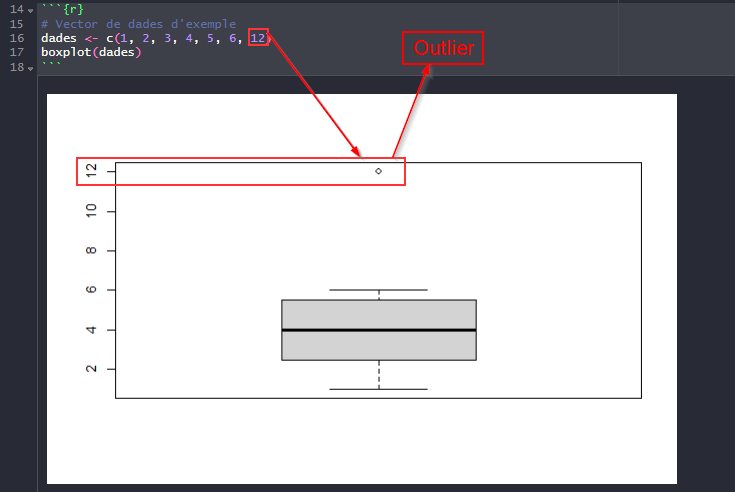
\includegraphics[scale=0.8]{images/boxplot.png}
    \caption{Exemple outlier diagrama de caixa}
    \label{fig:boxplot}
\end{figure}
\begin{figure}[h]
    \centering
    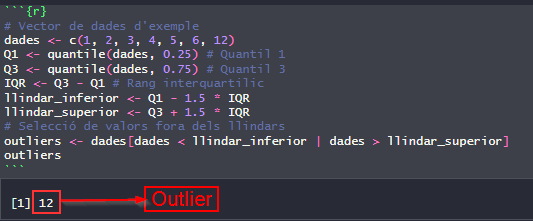
\includegraphics[scale=1]{images/iqr.png}
    \caption{Exemple outlier IQR}
    \label{fig:iqr}
\end{figure}
\begin{figure}[h]
    \centering
    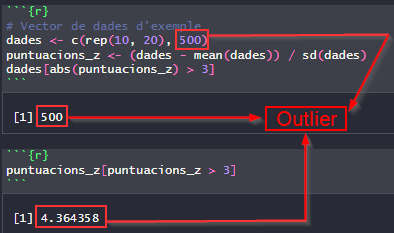
\includegraphics[scale=1]{images/z-scoring.png}
    \caption{Exemple outlier Z-scoring}
    \label{fig:zscoring}
\end{figure}
\section*{Exercici 2}
\addcontentsline{toc}{section}{Exercici 2}
\subsection*{Pregunta 1}
\addcontentsline{toc}{subsection}{Pregunta 1}
Les dades perdudes afecten (o poden afectar) l'anàlisi de les dades, ja que disminueixen la mida de les mostres vàlides i a conseqüència d'aquest fet, es redueix la força de comparació hipòtesis.\\
Existeixen tres tipus de dades perdudes: Les MCAR (\textit{Missing Completely Random}) que són aquelles dades en les quals la raó per la qual estan absentes és aliena a les mateixes dades. Les MNAR (\textit{Missing Not at Random}) que són aquelles dades en les quals la raó de la seva absència depèn precisament de les mateixes dades que s'han recollit. El tercer tipus de dades perdudes són les MAR (\textit{Missing at Random}) que són aquelles dades en les quals la raó de la seva absència no depèn de les mateixes dades perdudes, però que pot estar relacionada amb altres variables del conjunt de dades.\\
Per escollir la millor tècnica d'imputació cal tenir en compte la mida del \textit{dataset}, la proporció de variables afectades i la quantitat d'informació perduda.
\subsection*{Pregunta 2}
\addcontentsline{toc}{subsection}{Pregunta 2}
\subsubsection*{Imputació simple: Imputació utilitzant la mitjana o la moda}
És el mètode més senzill de tots i es basa a substituir els valors absents per la mitjana aritmètica de la variable si aquesta és contínua. En el cas de les variables categòriques, s'imputaria la moda.\\
Per exemple, per al primer cas es pot suposar que un \textit{dataset} conté la variable \textit{age} i que té dades perdudes. Doncs segons s'ha descrit, aquelles dades absents se substituirien per la mitjana de les edats informades en les dades. Un exemple per al segon cas seria que el \textit{dataset} tingui la variable \textit{gender}. En aquest cas s'imputaria en les dades absents la categoria més "popular".
\subsubsection*{Imputació simple: Regressió lineal}
Aquest segon mètode es basa a imputar utilitzant un model de regressió lineal per predir el possible valor de cada dada perduda.\\
Un exemple per aquest cas podria ser un \textit{dataset} d'informació dels treballadors d'una companyia en el qual falten dades del salari d'alguns treballadors. Es podria usar un model de regressió lineal per predir el salari a partir d'altres dades del treballador com: edat, càrrec, estudis, antiguitat a la companyia, etc.
\section*{Exercici 3}
\addcontentsline{toc}{section}{Exercici 3}
\subsection*{Pregunta 1}
\addcontentsline{toc}{subsection}{Pregunta 1}
La correlació entre dues variables és una mesura estadística que denota fins a quin punt dues variables estan relacionades linealment. Dues variables estan associades quan una d'elles dona informació sobre l'altra i dues variables es correlacionen quan tendeixen a créixer o decréixer.\\
El grau de correlació es descriu mitjançant una mesura, adimensional, que pot prendre valors compresos entre -1 i 1. Com més proper a 0 és aquest valor, més dèbil és la correlació lineal i com més proper a 1 o -1 més forta. Els valors positius indiquen que ambdues variables tendeixen a augmentar juntes i els valors negatius indiquen que una de les variables tendeix a augmentar mentre que l'altra tendeix a disminuir.\\
Un exemple podria ser un estudi de causes d'hipertensió arterial, que analitza la relació entre el consum diari de sal i la pressió arterial. Es plantegen els següents possibles escenaris:
\begin{itemize}
    \item Coeficient 1 $\longrightarrow$ L'augment del consum de sal s'associa sempre a l'augment proporcional de la tensió.
    \item Coeficient -1 $\longrightarrow$ L'augment del consum de sal, implica la disminució de la tensió.
    \item Coeficient $>$ 0 $\longrightarrow$ Tendència a un augment la tensió amb l'augment del consum de sal.
    \item Coeficient $<$ 0 $\longrightarrow$ Tendència a una disminució de la tensió amb l'augment del consum de sal.
\end{itemize}
\subsection*{Pregunta 2}
\addcontentsline{toc}{subsection}{Pregunta 2}
La regressió lineal s'utilitza quan la variable depenent és numèrica i s'assumeix que la relació entre la variable depenent i les variables independents és lineal. Per tant, és una tècnica que busca construir un model que expliqui la relació entre una variable depenent i les independents amb l'objectiu de trobar la línia d'ajust que minimitzi al màxim la suma dels errors quadràtics entre els valors observats i els predits.\\
Mètriques: \textit{R-squared}.\\
Un exemple de regressió lineal podria ser la predicció del valor d'una casa segons la superfície, el nombre d'habitacions banys, antiguitat, etc.\\
La regressió logística s'usa quan la variable depenent és categòrica i binària. En aquest cas, el que es busca un és un model que expliqui la probabilitat que tingui lloc un esdeveniment binari donant com a sortida una probabilitat entre 0 i 1.\\
Mètriques: \textit{Akaike Information Criterion}.\\
L'exemple en aquest cas podria ser la predicció de la probabilitat que un alumne aprovi una assignatura segons hores dedicades a l'assignatura, notes, classes ateses, etc.
\section*{Exercici 4}
\addcontentsline{toc}{section}{Exercici 4}
\subsection*{Pregunta 1}
\addcontentsline{toc}{subsection}{Pregunta 1}
L'aprenentatge supervisat es basa en un conjunt de dades d'entrenament perfectament etiquetades i classificades. És a dir, cada dada que es veurà durant la fase d'entrenament del model té una etiqueta que indica una única resposta correcta. L'objectiu d'aquest tipus d'aprenentatge és trobar patrons en les dades sense tenir informació prèvia sobre elles a part de la seva categoria. Durant la fase d'entrenament del model, aquest ha d'aprendre a trobar els patrons ocults en les dades de cada etiqueta perquè un cop entrenat sigui capaç de fer prediccions concretes sobre dades no etiquetades.\\
Un exemple que podria representar aquest tipus d'aprenentatge és la classificació d'imatges. En aquest cas concret es considera una classificació binària amb respostes "Càncer" i "No càncer". El model rebrà una imatge d'una tomografia computada de les tiroides d'una persona i haurà de classificar la imatge segons si aquesta persona pateix, o no, càncer de tiroides.\\
L'aprenentatge no supervisat utilitza dades no etiquetades i el procés d'entrenament no té cap mena de supervisió humana. En aquest cas, el model rep totes les dades barrejades i sense etiquetar de manera que el mateix model ha de ser capaç d'identificar patrons en les dades i discriminar-les en diferents categories.\\
Un exemple per aquest cas podria ser l'agrupació de clients d'una botiga segons el tipus de roba que compren. Aquest exemple seria útil per les persones del departament de màrqueting de la companyia per poder fer campanyes publicitàries.
\subsection*{Pregunta 2}
\addcontentsline{toc}{subsection}{Pregunta 2}
Precisió $\longrightarrow$ És la proporció de vertaders positius entre el total de positius (vertaders + falsos). Entenent com a "vertader positiu" els casos en què la predicció dona com a resultat que la dada en qüestió pertany a la classe X i realment pertany a la classe X. S'entén com a "fals positiu" aquells casos en els quals el model classifica una dada en una classe X, però aquesta dada realment correspon a una altra classe Y. Es calcula com el quocient del nombre de vertaders positius entre la suma del nombre del nombre de vertaders positius més el nombre de falsos positius.\\
\textit{Accuracy} $\longrightarrow$ És el percentatge de valors classificats correctament pel model. Es calcula com el quocient de la suma del nombre valors ben classificats (vertaders positius i vertaders negatius) entre observacions totals.\\
\textit{Recall} $\longrightarrow$ És la ràtio de vertaders positius i indica quants valors positius han estat classificats correctament. Es calcula com el quocient del nombre de vertaders positius entre la suma del nombre de vertaders positius més el nombre de falsos negatius.
\section*{Exercici 5}
\addcontentsline{toc}{section}{Exercici 5}
\subsection*{Pregunta 1}
\addcontentsline{toc}{subsection}{Pregunta 1}
La visualització de les dades és fonamental per identificar patrons, tendències, errors, anomalies i \textit{outliers} que podrien no ser detectats sense aquestes representacions gràfiques.\\
La primera de les representacions són els gràfics de barres. Aquests gràfics posen èmfasi a comparar elements.\\
Un exemple podria ser agafar com a població d'estudi tot l'alumnat d'ESO d'un institut, calcular les notes mitjanes de les assignatures i graficar-les en un gràfic de barres on cada barra representaria una assignatura. D'aquesta manera es podria identificar quines són les matèries amb pitjors resultats de tot l'institut.\\
La segona representació són els gràfics de línies que permeten veure com evoluciona una variable.\\
Un exemple podria ser durant la pandèmia de la COVID, el nombre de casos confirmats. És a dir, durant un temps X s'agafaria el nombre de casos confirmats diaris on cada punt representaria els malalts de cada dia. La forma de la línia permetria identificar patrons o tendències en el nombre de malalts.\\
La tercera tècnica són els gràfics de pastís que ajuden a veure com diferents parts representen un total.\\
Un exemple podria ser en un estudi sobre religió, un gràfic de pastís podria representar el percentatge de fidels a cada fe, essent el total la població mundial.
\end{document}
